\documentclass[10pt]{report}
\usepackage{graphicx}
\usepackage{bibentry}
\usepackage{enumerate}
\usepackage{multirow}
\graphicspath{{./Figure/}}
\title{
       
\includegraphics {ntu_log}
       REPORT 
        \center{ON 
        \center{INDUSTRIAL ORIENTATION 
        \center{WITH 
        \center{DATA STORAGE INSTITUTE
        }}}}}
\author{
        PREPARED BY :ZHANG SHU HAO\\
        \qquad\qquad U1022758E\\
        \quad        SCE
        }
\date{\qquad \qquad 11 July 2013}       

\begin{document}
	\bibliographystyle{plain}	
	\maketitle
	\newpage
	%
	\chapter*{Abstract}
	\addcontentsline{toc}{chapter}{Abstract}
		This report describes the working experience during my industrial orientation with Data Storage Institute. 
		During the period, I was assigned with the tasks that help to implement/ improve the current security storage system.
		Multi-tenant shared storage systems are foundation for the deployment of cloud storage service. With the popularity of cloud storage service, data protection in this multi-resource and multi-tenant environment becomes even more critical and challenging, among which performance degrading, operation complexity and scalability resulted from data protection using cryptal are the hottest issue. We proposed a high-throughput multi-tenant data protection over distributed storage system, providing low-penalty data protection mechanism for multi-tenant cloud storage with good scalability and transparent setup of data protection engine. 
		We further investigate the possibility of integrating security layer into current openstack project(grizzly). The integration of hardware encryption engine and new framework is left as future work.
		My contribution is twofold: \ 1) Accelerating Data Protection for multi-tenant storage\ 2) New cloud storage framework with security feature
	\newpage
	%
	\chapter*{Acknowledgement}
	\addcontentsline{toc}{chapter}{Acknowledgement}
		I would like to take this opportunity to express my gratitude to NTU and Data Storage Institute(DSI) for giving me the chance to fulfil my Industrial Orientation in DSI.\\
		I would like to express my thanks to the following people whom have helped me with my project during my attachment:\\\\
		Mr.Miguel Rodel Felipe, my IO supervisor, for guiding and providing me with high valuable suggestions when I encountered problems.\\\\
		Dr.Ren Shu Qin and Mr.Chen Shi Bin, research scientists from DSI, for providing me with various solutions regarding cloud security and cryptographic engine solutions.\\\\
		Dr.Chen Yong Zhen, research fellow from NUS, for great co-operation with me.
		Last but not least, I would like to thank my NTU Tutor, Ravi Suppiah for his assistance in agreeing to co-supervise the continual of my IO project.
	\newpage
	%
	\tableofcontents
	\newpage
	%
	\listoffigures
	\newpage
	% main part
	
	\chapter{Introduction}
		\section{Objective}
		This report covers the project done by me during the period of 20th May 2013 to 26th July 2010. It includes the knowledge and experiences I learnt during the development of the projects.
		
		\section{Company Profile-Data Storage Institude(DSI)}
		The Data Storage Institute (DSI) was established in April 1996 through the expansion of the Magnetics Technology Center founded in June 1992 by the Agency for Science, Technology \& Research, or A*STAR (then known as the National Science \& Technology Board) and the National University of Singapore (NUS). DSI is a member of the Agency for Science, Technology and Research (A*STAR), Singapore.
		The Data Center Technologies (DCT) Division was first established in July 2000. It was previously known as the Network Storage Technology (NST) Division but was recently renamed to DCT in December 2010. DCT aspires to be at the top of the information management and storage industry value chain by creating and developing innovative technologies and solutions for the data center and storage industry. Research done at the division primarily focuses on four key areas, namely, intelligent high performance large scale storage system; data management, protection and security; solid state storage; and storage system benchmarking and interoperability.
	\chapter{Project Specification}
		\section{Objective}
		we aimed at building upon a Intelligent, Scalable and Security  yet High Performance Cloud Storage System, which composed of two parts, namely: encryption engine and new cloud storage framework.
		My task basically involved in developing these two.
		\section{Background}
		Multi-tenant shared storage systems are foundation for the deployment of cloud storage service. With the popularity of cloud storage service, such as Amazon S3, Google Drive, and Microsoft SkyDrive and so on, data privacy and security issues are addressed, from which performance overhead, operation complexity and scalability are resulted. Secure, transparent yet light overhead protection solution is highly demanded as a middleware on cloud storage.
		Data leakage in a large scale shared storage system can be classified as two aspects: 1) Tenant-to-tenant threats to peep or violate the neighbor guests' data; 2) Cloud-to-tenant threat to peep or violate the guests' data by taking advantage of data holder. With these threats, data isolation and privacy preserving are key challenges for multi-tenant storage systems against data leakage.
		There are two architectures proposed against these attacks on cloud storage. One is to enforce security mechanism such as encryption and access control on service provider; the other is to enforce on client’s site. The former architecture is based on the assumption of trusted cloud storage service which is not well acceptable. The later architecture introduces operation complexity to end users and contradicts the advantages of cloud storage.
   		Based on the attacks existing on cloud storage with multi-resources and multi-tenants, we have been working on efficient data protection and access control mechanism by keeping the scalability, convenience and utilization of cloud storage 			service. We proposed a collaborative architecture to let data owner (tenant) and data holder (service provider) to work together and defend the attacks mentioned above. Since cloud storage service provider has powerful yet cheaper facilities, 			data isolation and access control are enforced on provider side, but the data owner can still hide the exact policies and let storage provider to execute the access control.  For protecting data itself, we proposed a secure gateway for each 		  		organization to encrypt/decrypt data when putting/getting to/from cloud storage, yet this encrypt/decrypt procedure is transparent operation from end user viewpoint.
		Openstack\cite{openstackwiki}, as a open source project gathering attention from every aspects, through deeply understanding of the current structure of openstack, we found that, there's a lack of security layer in block storage. There is a project under development \cite{volumeencryptionwiki} trying to address this issue as we could be noticed through openstack community, while we purpose a new approach that can gain multiple advantages, I will get back to this in Ch.4. 
		
	%\fontsize{15}{15}\selectfont 
	\chapter{Hardware Driver Engine}
		\section{Preliminary Works}
			\subsection{From device mapper to device driver to FPGA}
			The transparent data protection workflow can be completed through device mapper, such as dm- crypt \cite{4,5}. Dm-crypt is a transparent disk encryption subsystem. It is part of the device mapper infrastructure, and uses cryptographic routines from the kernel's Crypto API. dm-crypt is implemented as a device mapper target and may be stacked on top of other device mapper transformations. It can thus encrypt whole disks (including removable-media), partitions, software RAID volumes, logical volumes, as well as files. It appears as a block device, which can be used to back file systems, swap or an LVM physical volume.
			The dm-crypt device mapper target resides entirely in kernel space, and is only concerned with encryption of the block device - it does not interpret any data itself. It relies on user space front-ends to create and activate encrypted volumes, and manage authentication. Such front-ends currently available include cryptsetup and cryptmount. We choose cryptsetup as our front end which is used to conveniently setup dm-crypt managed device-mapper mappings. LUKS \cite{5} for dm-crypt is implemented in an enhanced version of cryptsetup. LUKS is the standard for Linux hard disk encryption. By providing a standard on-disk-format, it does not only facilitate compatibility among distributions, but also provides secure management of multiple user passwords. In contrast to existing solution, LUKS stores all setup necessary setup information in the partition header, enabling the user to transport or migrate his data seamlessly, based on above reason, we use cryptsetup-luks extension as the project tool.
			Device-mapper crypt essentially target provides transparent encryption of block devices using the kernel crypto API, however due to the limitation of software performance, we are proposing a way of shifting the crypt work to high speed, fully pipelined FPGA card. To connect the dmcrypt device mapper with FPGA device, new device driver is designed and implemented.
			\subsection{Performance Related Issues}	
				\begin{enumerate}
				\item \textbf{Data Transaction and Transfer.} Programmed input/output (PIO) vs. Direct Memory Access (DMA). PIO modes require a great deal of CPU overhead to configure a data transaction and transfer the data compared with DMA. System performance is heavily affected by PIO. To maximize the efficiency of DMA, PIO instructions are avoided if possible.
				\item \textbf{Crypto Block Driver.} Synchronous block driver vs. Asynchronous Driver [texbookCrypto]. Synchronous block driver makes cipher process block by block serially, which decrease the chunk data throughput. Asynchronous block driver could let FPGA based cryptographic engine pipelining with the device mapper to enhance total throughput tremendously.
				\item \textbf{Multiple DMA Channels. }With the data direction to and from FPGA device, at least two channels for each transaction could exploit the duplex nature of the PCIe link.
				\end{enumerate}
				\begin{figure}[ft]
				\includegraphics[width=\textwidth,height=\textheight,keepaspectratio] {fig1}
				\caption{Data Protection System for Multi-tenant Storage}
				\label{Figure 1}
				\end{figure}
		\section{High-throughput Data Protection for Multi-tenant Storage}
			\subsection{System Architecture}
				This system is to protect data for multi-tenant cloud storage where data flow from multiple computing servers at different organizations. A collaborative solution is deployed to ensure secure and high performance cloud storage. Two security aspects are to be addressed and enforced in a server- client collaborative way: 1) Secure Data Asset Management on Large Scale Shared Storage System to emphasize secure data access control; 2) Accelerating data protection for Large shared storage to emphasize high performance data crypt processing.				
			\subsection{Secure Data Asset Management on Large Scale Shared Storage System}
				Since the cloud storage provider is the data holder for multiple clients, data isolation and access control executed on service site would be efficient and feasibility to both clients and service provider. With data isolation and access control \cite{7,8}, guest-to-guest attack and guest-to-cloud attack can be eliminated. Still, the enterprise doesn't want to release its access control policies to the service provider. How can service provider provide a secure data access control satisfied by clients? We applied attributes based access control with our previous work on privacy preserved key words searching \cite{1}. By this, enterprise can hide its original attributes and set the encrypted attributes based access policies on cloud storage side. And the storage provider can implement and deploy access control on these privacy preserved attributes. The dataflow can refer Figure\ref{Figure 2} with step 1 to 5: 1) Organization A set access policy based on some attributes; 2) These attributes will be encrypted into meaningless attributes A1, A2 and so on; 3) based on these encrypted attributes, the corresponding access policy can be set on storage service provider who doesn't know the original attributes but still can assess whether that attribute meet or not; 4) The Policy Manager deploy its privacy preserved attributes to its staffs; 5) When staffs from the enterprise access storage, storage server has access proxy to check its corresponding privilege.
			\subsection{Accelerating data protection for Large shared storage}
				Besides secure data isolation and access control, we also investigated to accelerate data protection procedure to eliminate the latency brought in and minimize the operation complexity. Since data means value to enterprise, data protection by encryption has to be done before delivering to the cloud. To remove the operation complexity, we propose a secure gateway to do data protection for the enterprise data. Every staff's data will be encrypted automatically before going to the storage cloud; it is completely transparent to the staff without any operation enforced on the staff's computer. However this centralized mechanism brings in I/O performance and the corresponding latency issue. To eliminate the bottleneck and performance penalties caused from data encryption, a series of accelerating processes are deployed on the secure gateway. By incorporating hardware crypt task and pipelining process with software, the hardware performance is nearly made full usage of to speed up 4 times compared to the traditional mechanism. We also built a prototype to test out the practicality and feasibility. The positive results show its obvious improvement on big throughput and low latency support.
				\begin{figure}[ft]
				\includegraphics[width=\textwidth,height=\textheight,keepaspectratio] {fig2}
				\caption{Dataflow of Secure Data Access Control}
				\label{Figure 2}
				\end{figure}
			\subsection{Asynchronous Block Driver Design And Setup}
			As mentioned in Preliminary Works, with the poor performance of crypto API, new device driver is desired to connect device mapper and FPGA device to give high speed cipher process. To eliminate the performance penalty caused by protection, FPGA based encryption engine is designed and implemented. Since the cipher process shifted to FPGA, minimizing the cost of data transfer data between CPU and FPGA has tremendous influence on the performance. For the default synchronize block cipher, request is sending from device mapper with all information extracted and cipher process is done on each 64 Bytes serially, introducing high delay and communication cost. To enhance the performance, bigger block transfer and asynchronous block cipher are new designed and implemented.
			However for an asynchronous request is only a pointer to a request structure managed by device mapper cryptsetup, thus it must first extract the data to cipher; we called this phase as Dataprepare, controlled by thread Q-man to prepare multiple blocks of data. The second phase is to send bigger chunks of data for ciphering process, managed by D-man. The last phase is to pull status from H/W to adjust the index of block to process. With these three loosely dependent threads, pipelined processing is enforced as Figure \ref{Figure 3}, to further accelerate the cipher process.
				\begin{figure}[ft]
				\includegraphics[width=\textwidth,height=\textheight,keepaspectratio] {fig3}
				\caption{High Throughput Data Encryption with Pipelined Asynchronous Block Cipher Driver}
				\label{Figure 3}
				\end{figure}
			\subsection{Accelerating Asynchronous Block Driver}
			Considering the bottleneck step of DMA read and AES module, two different optimizations are deployed as following: 1) Split DMA read operation into two substage: send DMA read request and receive complete data sending package from CPU; 2) Incorporate two FIFO for pingpang operation on encryption module. AES module takes data from ingress fifo and then do cipher processing for about 20 cycles, two-FIFO pingpang operation can eliminate this bottleneck to 10 cycles. With these two optimizations, pipeline efficiency could be close to 1 with big data protection.
			To fully use the feature of pipeline working style of H/W, the device driver is further developed to expand the buffers and let the buffers working as a circular list, where each slots contain index associated with H/W frame slots, and temp pointer point to corresponding request waiting to be processed, as Figure \ref{Figure 4}.
				
				\begin{figure}[ft]
				\includegraphics[width=\textwidth,height=\textheight,keepaspectratio] {fig4}
				\caption{Ring buffer to accelerate cipher}
				\label{Figure 4}
				\end{figure}
			
			\subsection{Cylinder architecture for multiple FPGA}
			Due to the effect that each request contains all necessary information, it's possible to further create multi-channel DMA to further eliminate the data transfer delay. Based on the ring architecture illustrated above, the driver can further extend to Cylinder architecture version by extend current structure into multi- dimensions array structure, each ring structure corresponding to one FPGA card, with multiple FPGA card or multiple processes on one FPGA card, the performance will be further increased.
		\section{Experiment Results and Analysis}
			\subsection{Experiment Setup}
			In our system, two normal computers with 8x PCIe slot is used as an encryption engine and a key manager. On the encryption engine machine, a Xilinx ML605 Demo board with virtex 6 FPGA chip is used for the FPGA-based encryption. We did data protection performance test on 4KB data.
			\subsection{Comparison among software encryption, device driver with FPGA, optimized driver with FPGA}
			First, we check the throughput performance without encryption on 4KB data as the baseline, and get the result of 235MB/s for reading and 197MB/s for writing. With this baseline, we did throughput test with software based data encryption, default synchronous device driver with FPGA-based encryption and asynchronous device driver with FPGA-base encryption: 1) For software based data encryption, throughput test is done using dd utility to read and write 4KB data block, then device mapper dm-crypt calls the crypto API to encrypt data, the maximum throughput is 74.3MB/s for reading and 60.9MB/s for writing; 2) For asynchronous device driver pipelined with FPGA-based encryption, the throughput on device driver can go for 367MB/s and the throughput with dd utility is 193MB/s for reading and 134MB/s for writing.
			\section{Future Works}
		We create a hardware solution to speed up data protection. Possible future works to improve the performance:
		\begin{enumerate}
				\item Setting interrupt scheme with hardware, thus reduce cpu burden of polling check status register.
				\item Instead of change status number, let hardware directly change CTI pointer (i.e. modify address of CTI), thus the reading of status and updating of CTI can be combined together.
				\item Instead of using only one FPGA card, upgrade to multiple FPGA card, or one FPGA card with multiple thread concurrently processing.
				\item With RAID support, concurrently processing on multiple disk, further increase performance.
				\item Instead of Copy end data from SG list to a linear buffer and send this linear buffer to device, using dmamapsg directly send sg list to device, this will reduce overhead on CPU sufficiently but require necessary hardware support.
				\item Coming from the idea that dmcrypt may be stacked on top of other device mapper transformations. We may create another general driver layer sitting in between dm-crypt and specific driver.
		\end{enumerate}
	\chapter{Security Cloud Storage Framework}		
		\section{Preliminary Works}
			\subsection{OpenStack}			
			\paragraph{\large Openstack}
			 is being properly documented and maintained with communities' great effort, however,for someone planning to get involved, it's still difficult to understand the implementation detail and physiology behind the scene.
			To quickly step into the deep, I read the source code and drew UML diagrams for some of the most important functions, including:
			\begin{enumerate}
				\item service,Figure \ref{service}, shows how service(nova-api,nova-sch,cinder-vol,cinder-sch,etc) are starting, and the  related files.
				\item manager,Figure \ref{manager}, shows the inner struct of manager class.
				\item runInstance,Figure \ref{runInstance}, shows the workflow of creating instance.
				\item createVolume(cinder Part), Figure \ref{cinder}, shows the workflow of creating volume in cinder side.
				\item createVolume(nova Part), Figure \ref{nova}, shows the workflow of creating volume in nova side, this is unnecessary in many cases, I will explain this more in next paragraph.
				\item attachVolume(nova-cinder),Figure \ref{attach}, shows the workflow of creating volume in nova side, this is unnecessary in many cases.
			\end{enumerate}
			\begin{figure}[!htbp]
				
				\includegraphics[width=\textwidth,height=\textheight,keepaspectratio] {runInstance}
				\caption{Nova run instance}
				\label{runInstance}
			\end{figure}
			\begin{figure}[!htbp]
				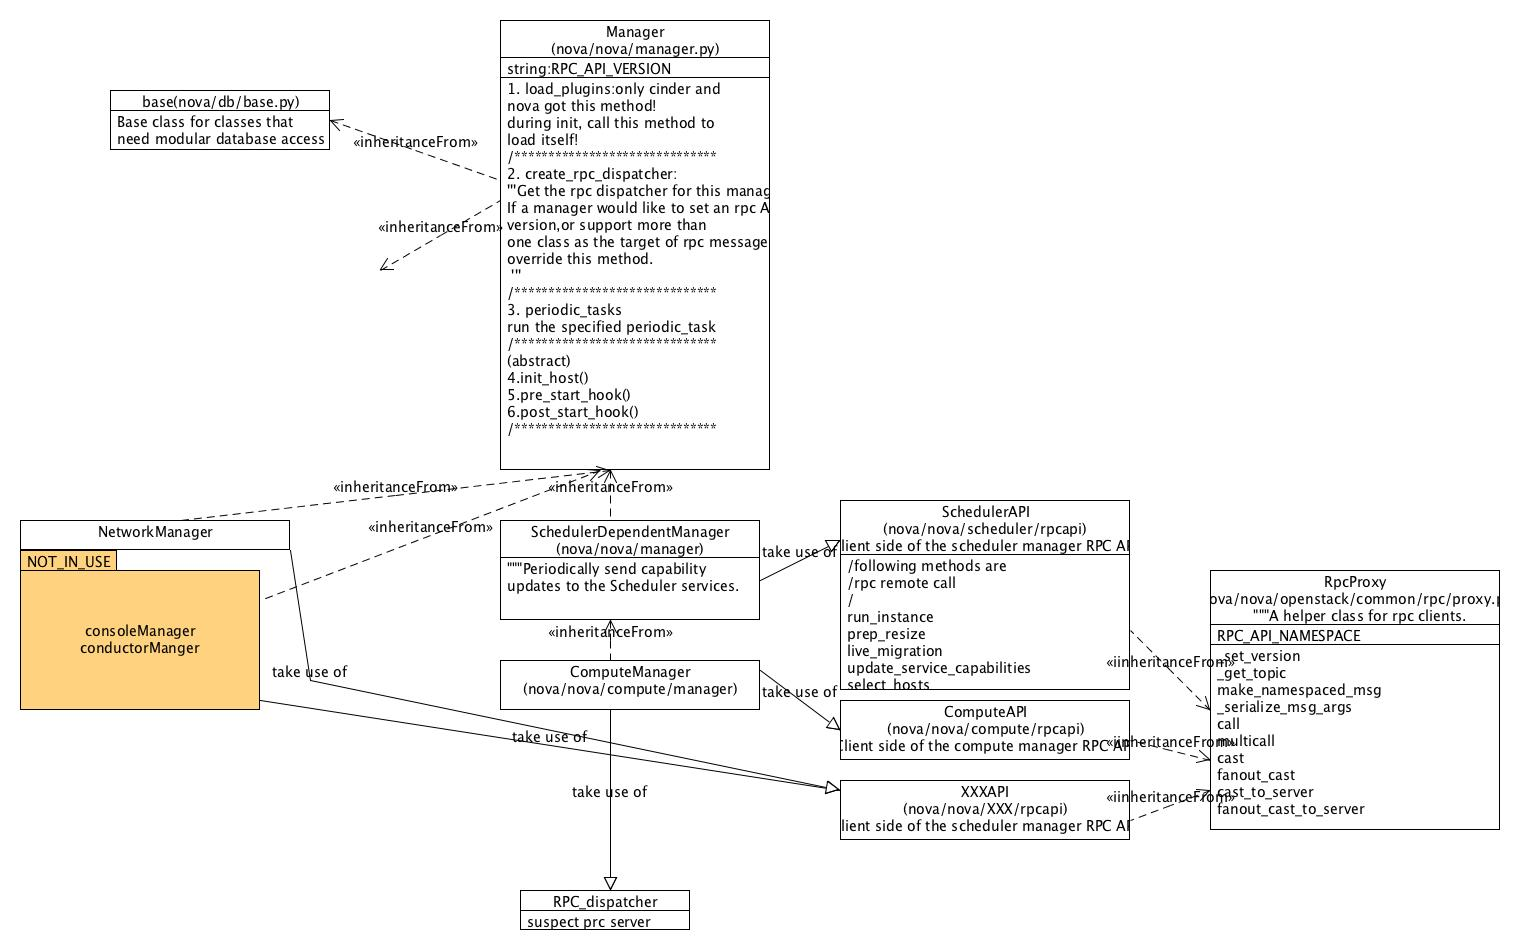
\includegraphics[width=\textwidth,height=\textheight,keepaspectratio] {Manager}
				\caption{GeneralManager structure}
				\label{manager}
			\end{figure}
			\begin{figure}[!htbp]
				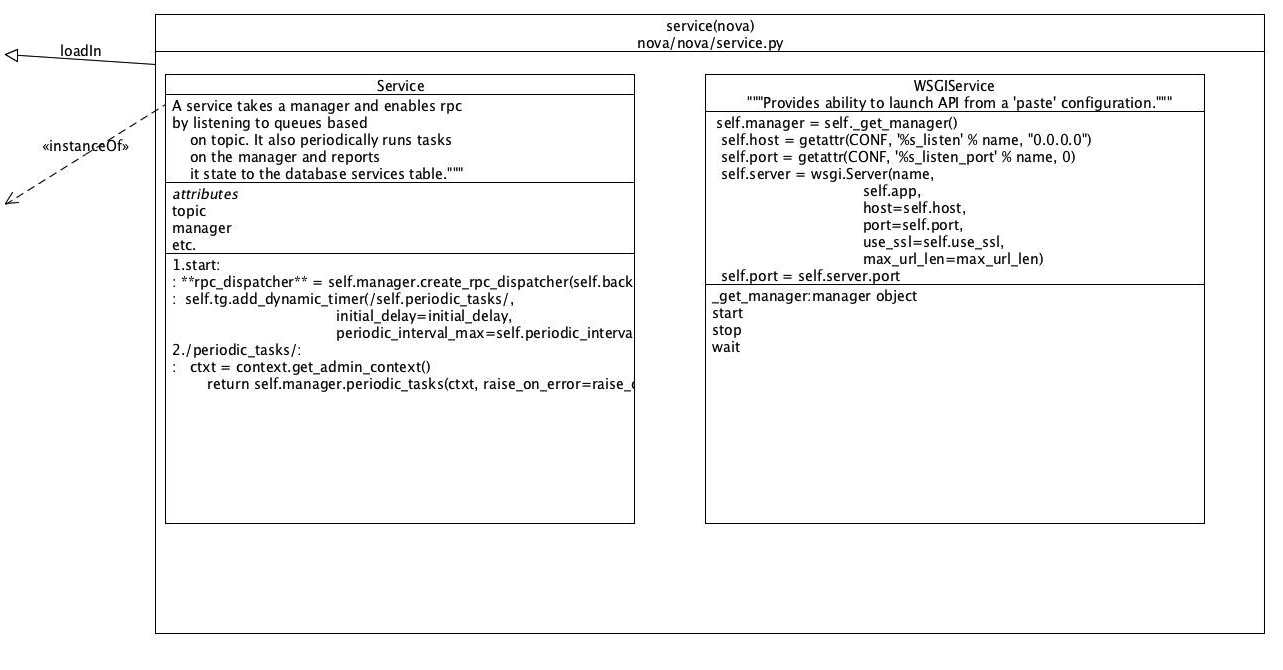
\includegraphics[width=\textwidth,height=\textheight,keepaspectratio] {service}
				\caption{GeneralService starting}
				\label{service}
			\end{figure}
			\begin{figure}[!htbp]
				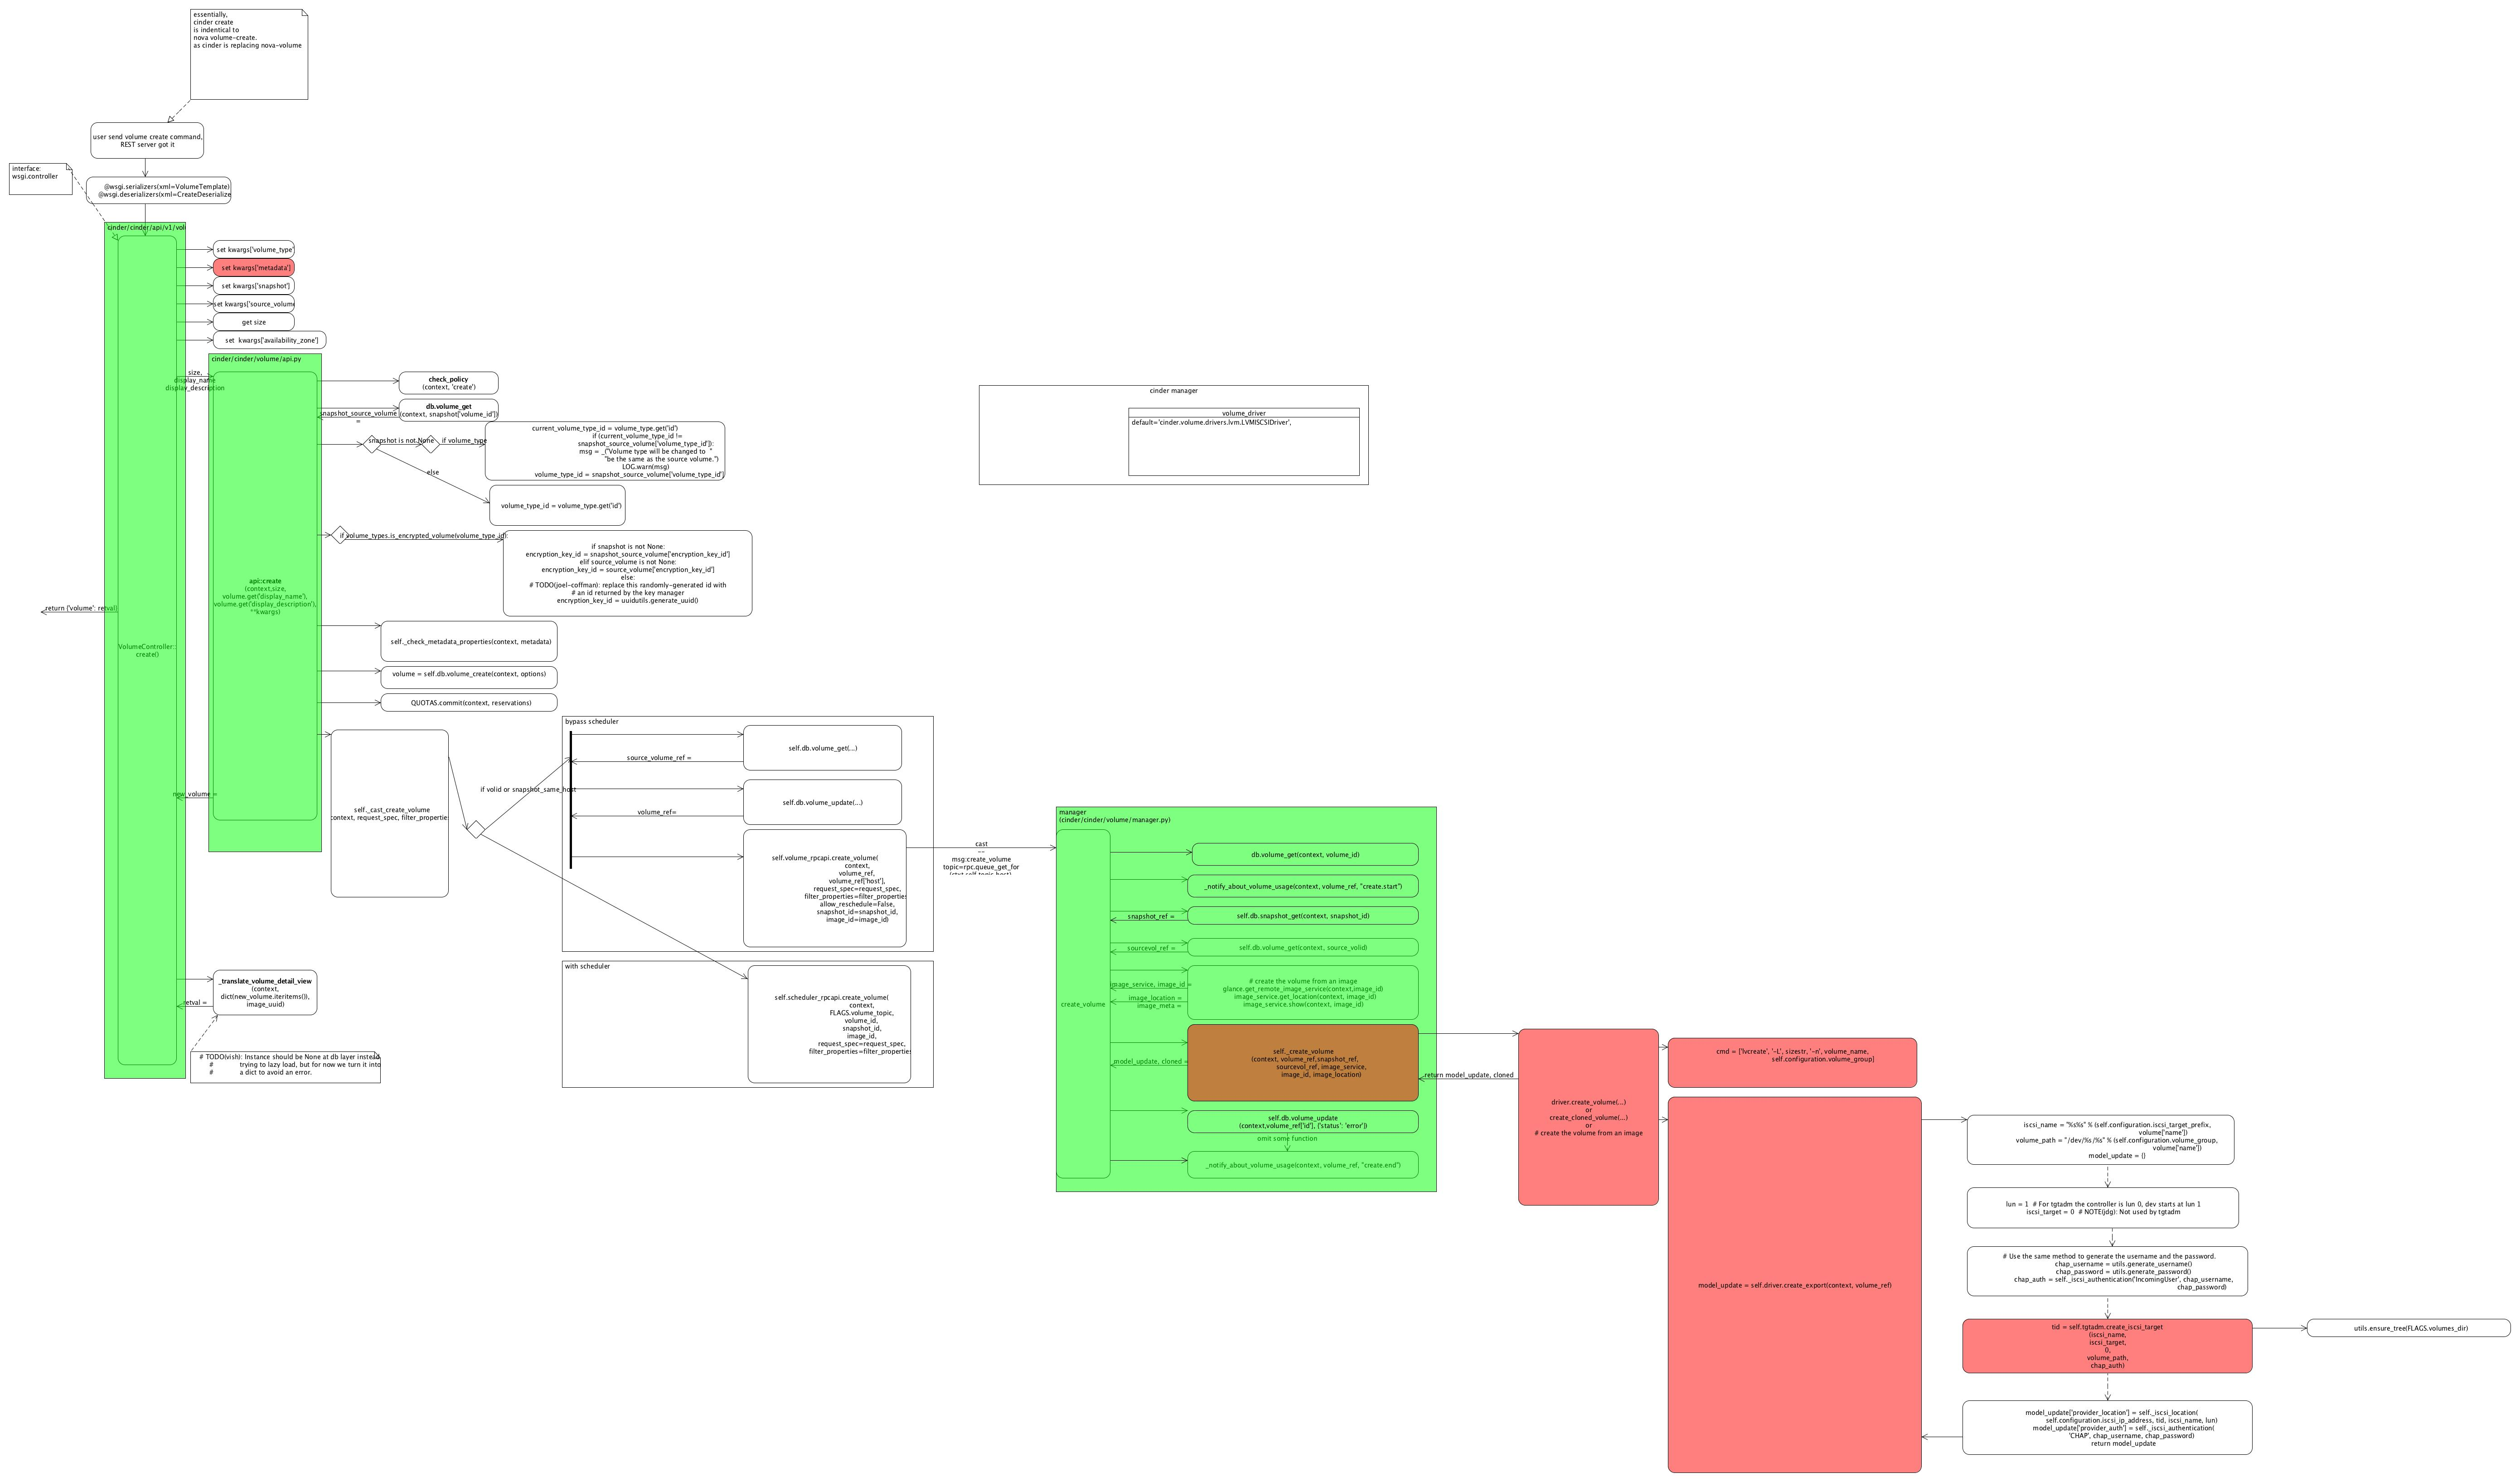
\includegraphics[width=\textwidth,height=\textheight,keepaspectratio] {cinder}
				\caption{volumeCreation-cinder}
				\label{cinder}
			\end{figure}
			\begin{figure}[!htbp]
				\includegraphics[width=\textwidth,height=\textheight,keepaspectratio] {nova}
				\caption{volumeCreation-nova}
				\label{nova}
				\end{figure}
			\begin{figure}[!htbp]
				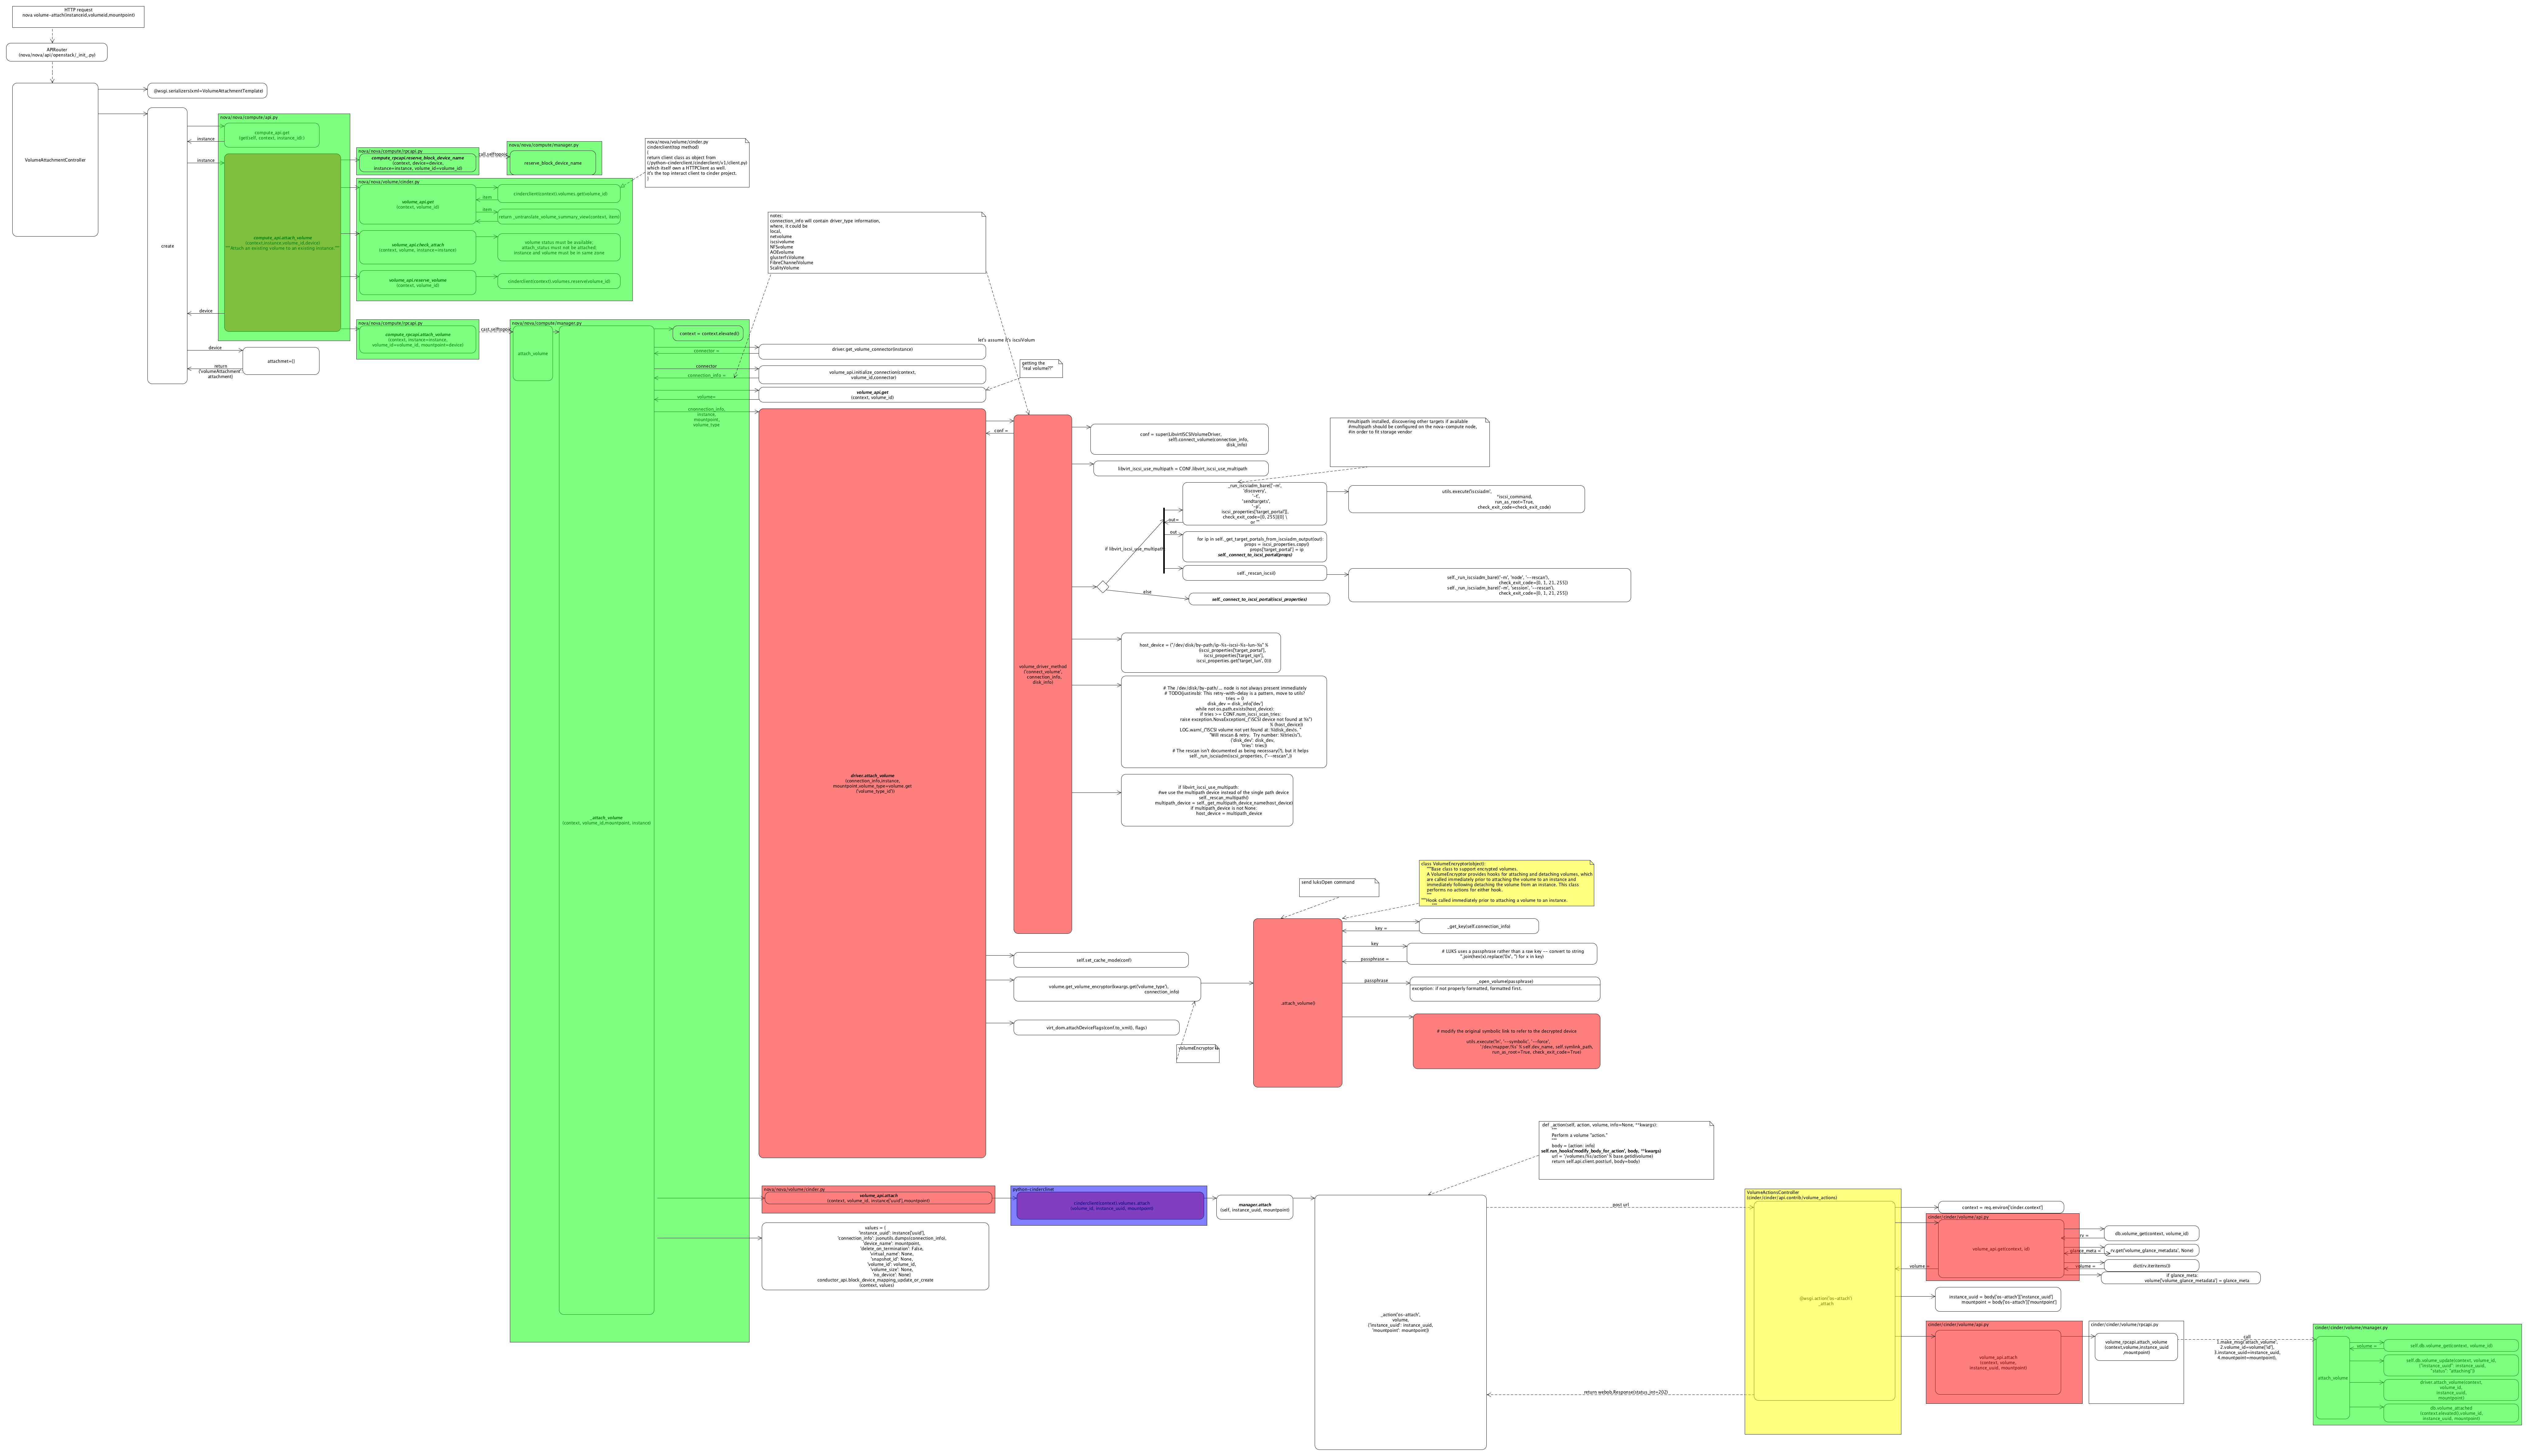
\includegraphics[width=\textwidth,height=\textheight,keepaspectratio] {attach}
				\caption{volumeAttach}
				\label{attach}
			\end{figure}
			\newpage
			\paragraph{\large communication} can be classified into  two main parts:
			\begin{enumerate}[$\bullet$]
				\item  \textbf{rpc communication}( API $\rightleftharpoons $Manager), rabittmq as backend server, "API"(as client) can communicate(send request, either cast/call) to Manager, meanwhile, Manager can take use of "API" to communicate with other Manager. 
				\item  \textbf{http communication}( wsgi client of one service $\rightleftharpoons $wsgi server of another service), for instance, when nova want to attach volume to it's instance, it need to communicate with keystone to prove it's identity and then send signal to cinder, in which, two http request happens.
			\end{enumerate}
			\subsection{Secruity Gateway(aka. proxy)}
			Based on openstack, we investigate the possibility of building security cloud storage system, please refer to Figure \ref{iscsiplan}. 
			\begin{figure}[fhtbp]
				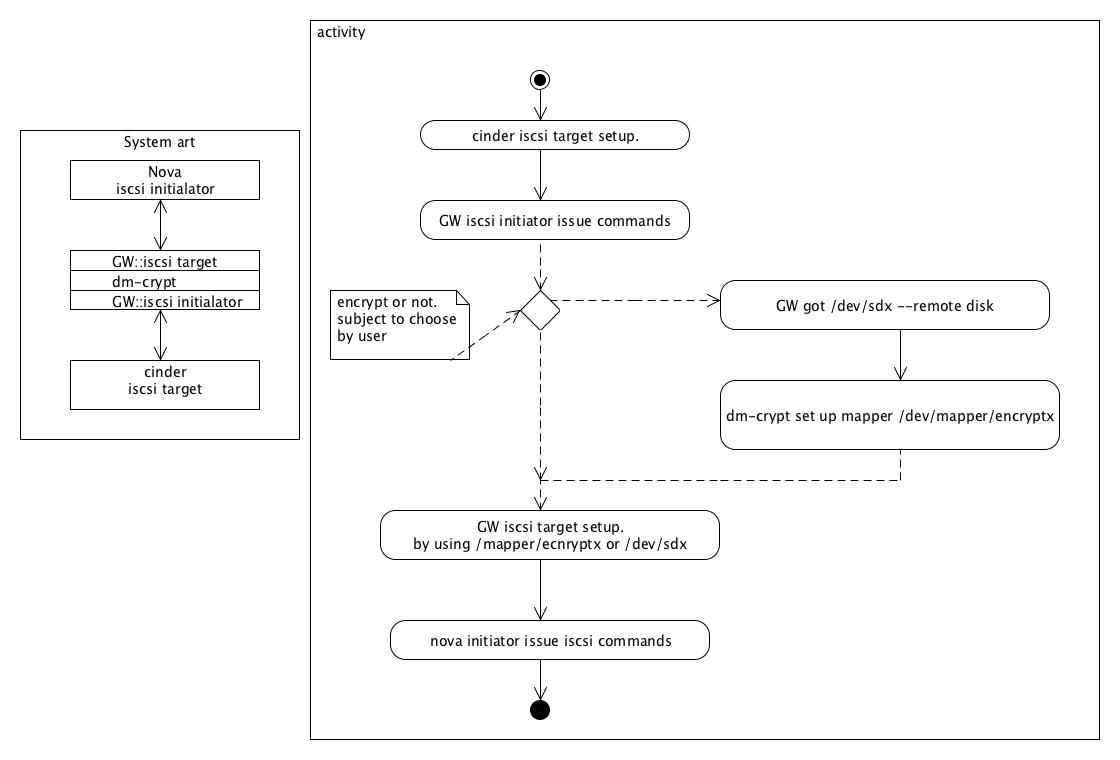
\includegraphics[width=\textwidth,height=\textheight,keepaspectratio] {iscsi(plan)}
				\caption{GateWay Design}
				\label{iscsiplan}
			\end{figure}
			\newpage
			\subsection{Main Implementation}
			Implementation involved two stages: 
			\begin{enumerate}[$\bullet$]
			
			\item 
			\textbf{manual testing:} setup three nodes: node1: nova+keystone+quantum; node 2 : gateway; node 3 : cinder.
			\paragraph {\ \ volume creation, encryption volume creation:}
			in node 3: Issue $"cinder\ create --size\ 1"$ to create logic volume on cinder(original), since it will automatically export iscsi target, the work on it is done. The equivalent command is:
			$lvcreate ->  tgtadm -op new ->  tgtadm --bind.$
			in node 2: Issue $" iscsiadm --mode discovery -> iscsiadm --mode node -> cryptsetup\ luksFormat -> cryptsetup\ luksOpen -> tgtadm --op\ new -> tgtadm --bind .$
			in node 1: Issue "cinder create", when gateway received signal, it will make a symbol link to the just created encrypted volume, till here, all operation done.
			\paragraph {\ \ instance creation and volume attach:}
			in node 1:Issue $"nova\ boot --image <uuid> --flavor m1.tiny --key_name test --availability-zone nova:server2"$, $nova\ volume\ attach --server xx --volume xx$. Till here, all operation related is done.
			\item 
			\textbf{automatic testing:}
			to make above operations automatic, we need to embed some commands into python code of original cinder, some of challenges are: \\ volume creation signal from node 2 forwarding to node 3, which may result in error in node 3 and have to retry in node 2 ; after iscsi login, it's unknown to know which partition is created locally, I use $ls -lart /dev/disk/by-path | awk '{print \$9 " " \$11}' | grep \$targetname | awk '{ print \$2 }'  $ to find the correct one, which is not optimised yet.\\
			Most of the change happened in Gateway side, please refer to Figure \ref{GWcreate}.
			
			\end{enumerate}
			\begin{figure}[fht]
				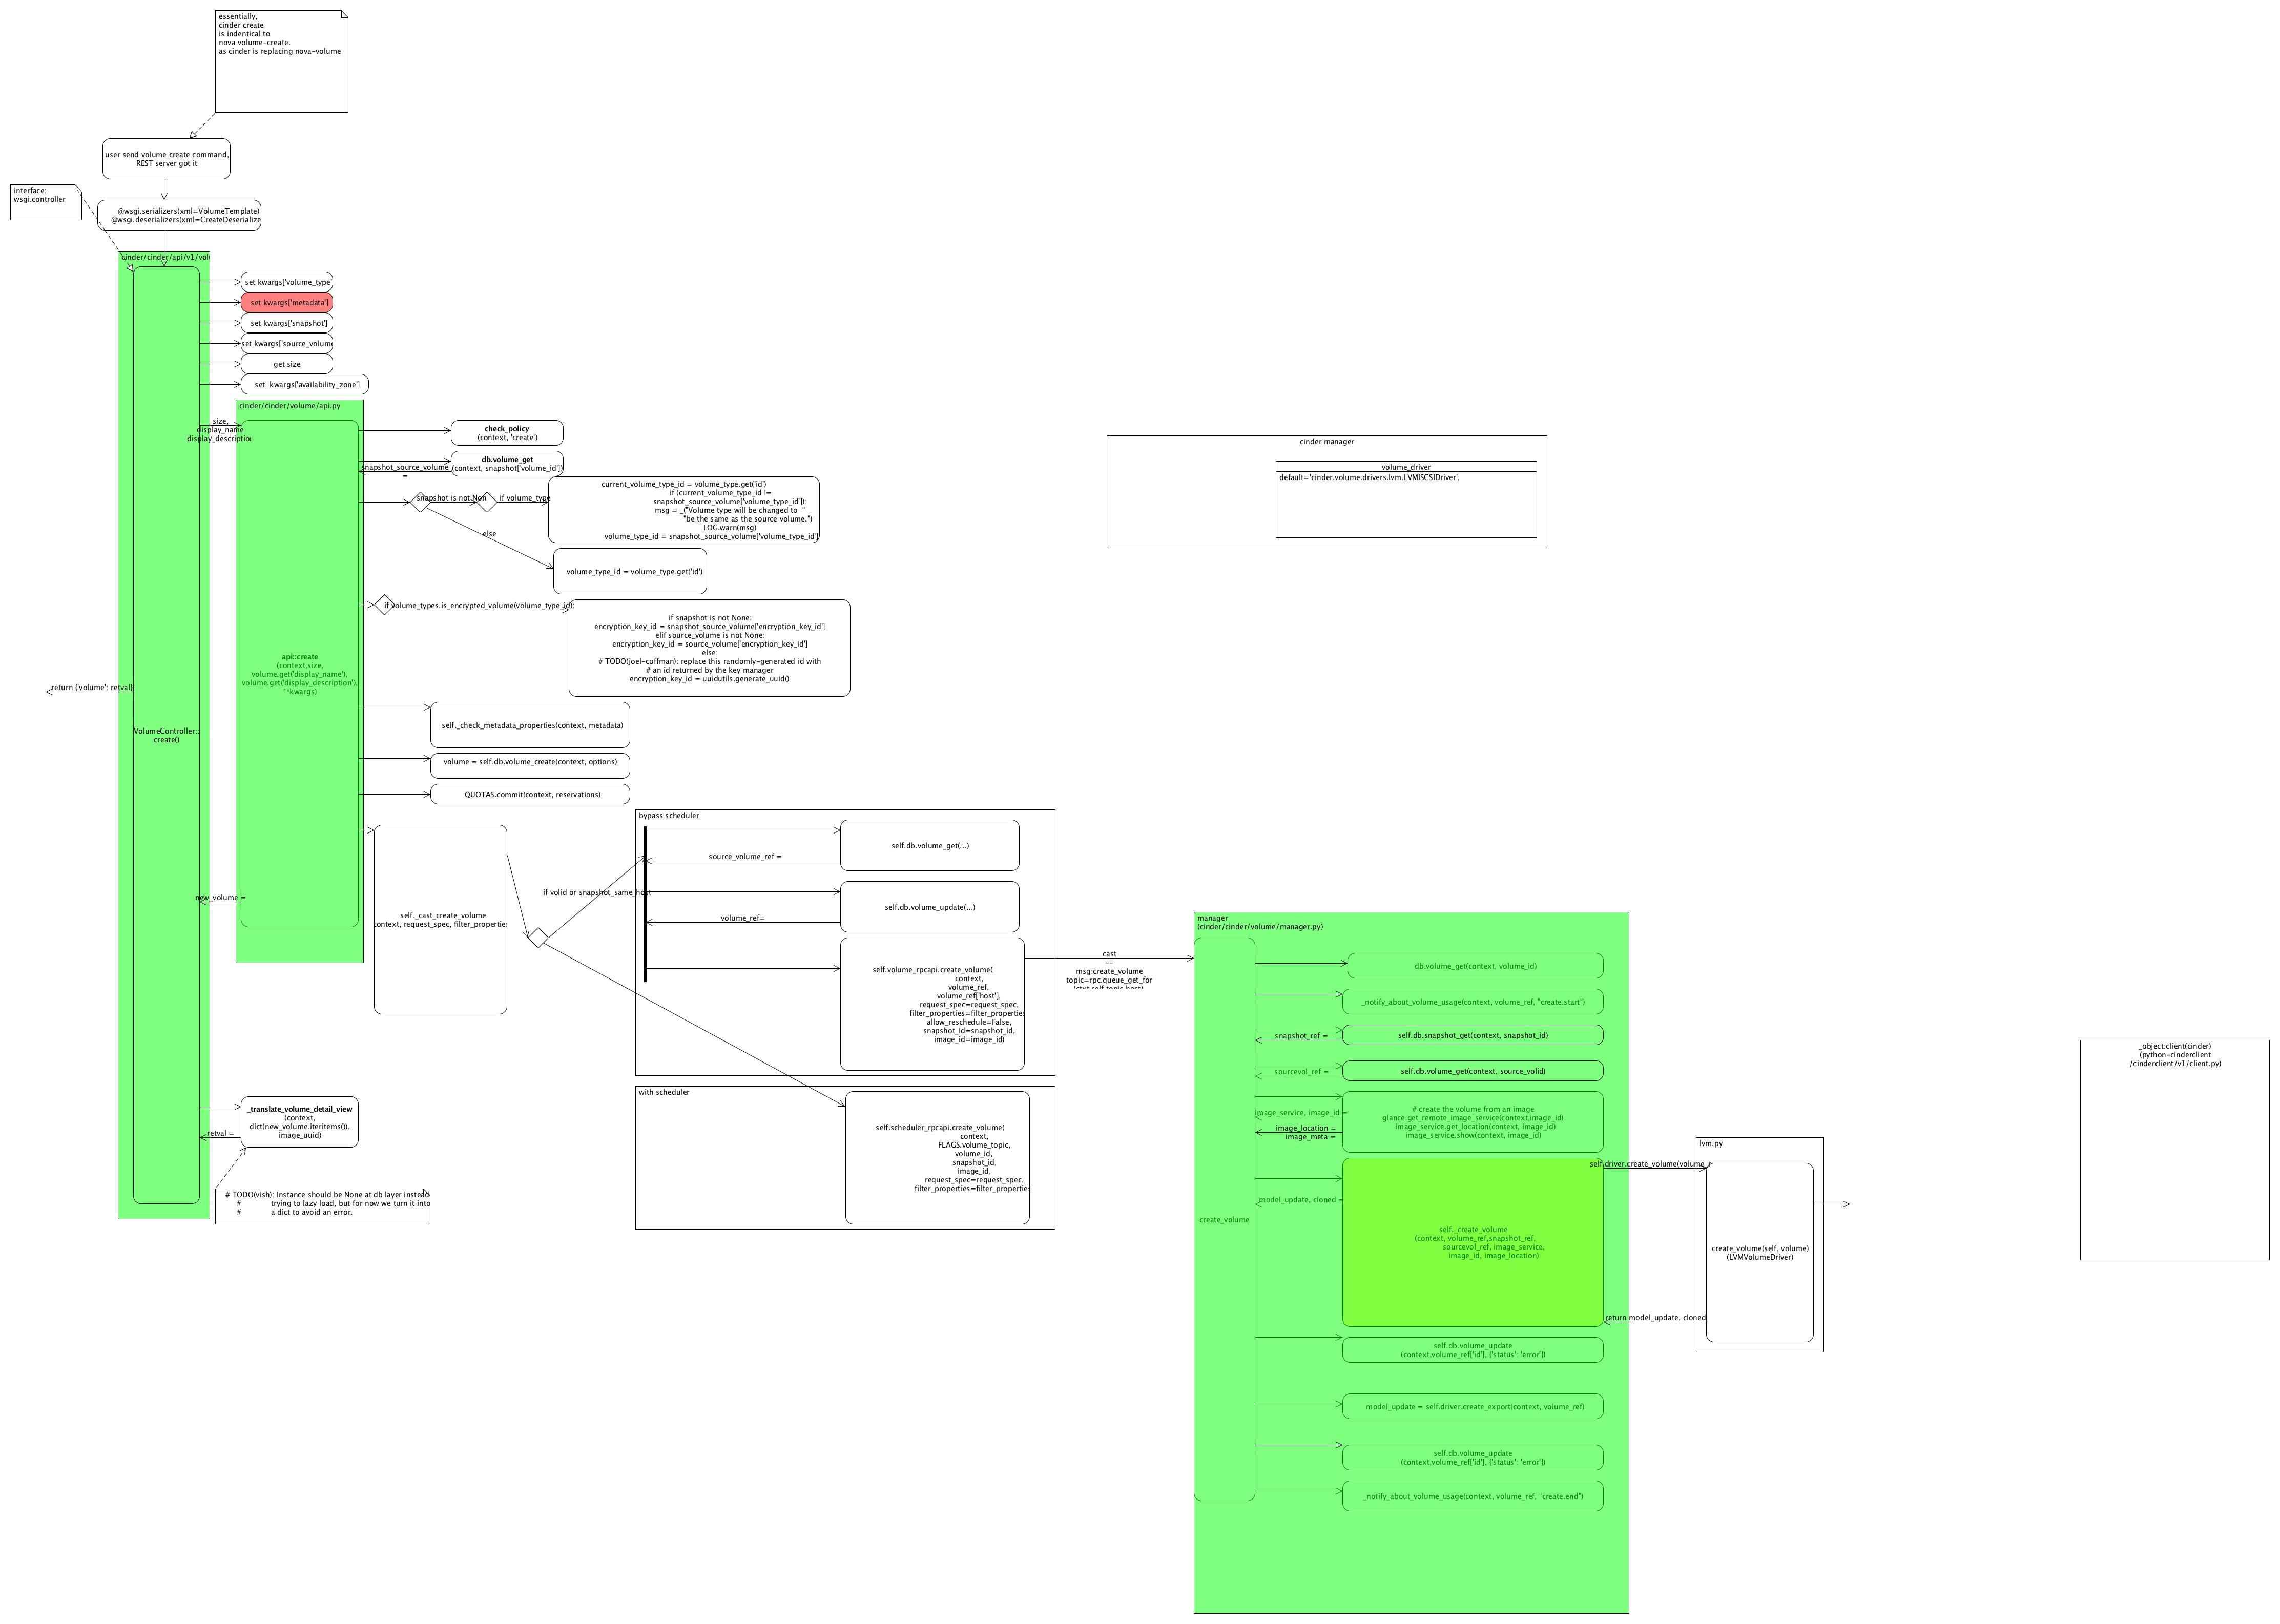
\includegraphics[width=\textwidth,height=\textheight,keepaspectratio] {GW-createvolume}
				\caption{GateWay create volume}
				\label{GWcreate}
			\end{figure}
			
			\section{Experiment Results and Analysis}
			\subsection{Experiment Setup}
			The purpose of this section is to provides steps that allow developers to get an environment where they can test out the volume encryption feature. It also provides guidance on how to execute the feature and manually verify that it is working.
			We setup openstack environment through devstack and we assume cryptsetup is pre-installed. The main change you need to manually setting is as following:\\
			\textbf{Environment pre-setting}\\
			enable all services in localrc and run stack.sh to properly configure all related environment.\\
			\textbf{Keystone register configuration:}\\
			
			in\ node\ 1:$python-cinderclient/cinderclient/v1/clien.py: line 86: service\_type = "GWvolume'$\\
			$nova/nova/volume/cinder.py line 92, change service\_type to "GWvolume"$\\
			$python-cinderclient/cinderclient/service_catalog.py\ line\ 62\ change service\_type to "GWvolume"$\\
			
			in\ node\ 2 : $python-cinderclient/cinderclient/v1/clien.py:line\ 86: service\_type = "Purevolume'$,\\
			$ devstack/lib/cinder, line\ 294: change\ type\ to\ GWvolume.\\$
			$line\ 270\ add\ export\  OS\_AUTH\_URL="http://\$keystoneIp:5000/v2.0" \\$
			$export\ OS\_USERNAME=admin \\$
			$export\ OS\_PASSWORD=password \\$
			$export\ OS\_TENANT\_NAME=admin\\$
			
			in\  node\ 3:  $python-cinderclient/cinderclient/v1/clien.py: line\ 86: service\_type = "Purevolume'$,\\
			$ devstack/lib/cinder, line\ 294: change\ type\ to\ Purevolume. \\
			line\ 270 add\ export\  OS\_AUTH\_URL="http://\$keystoneIp:5000/v2.0" \\$
			$export\ OS\_USERNAME=admin \\$
			$export\ OS\_PASSWORD=password \\$
			$export\ OS\_TENANT\_NAME=admin$\\
			\textbf{Localrc setting:}\\
			Set localrc of node 1 to enable all but cinder service, Set localrc of node 2 and node 3 to enable only cinder service.\\
			start to run all node in sequence of node 1, node 2, node 3, through run ./stack.sh.	It might take a few retires, check log for any error occur\\	
			work through in node 1 host:\\
			\textbf{Other modification:}\\
			in\ node\ 2: $stack.sh\ line\ 862\ add\  create\_cinder\_accounts;$\\
			in\ node\ 3:$stack.sh\ line\ 862\ add\ create\_cinder\_accounts$, replace the /opt/stack/cinder as the modified version. \\
			Remember to change /cinder/cinder/volume/PCAPI.py line 97 and lvm.py line 213, 239
			according to current keystone services and cinder service ip address. Later should be upgraded to automatically setting.\\			
			\textbf{Test Setup Guide} \\
		
			\begin{enumerate}
			\item Create volume from nova site: unencryption volume created in cinder and encryption volume created in gateway.\\
			after above configuration is done, issue $cinder\ create\ 1$ in node 1, and wait until all operations done.\\
			you can use $cinder\ list$ to check current status.
			\item Iscsiadm login to these two different volume. (*Due to single point connection feature of iscsi, when node 3 connect to node 2, 
			node 1 cannot connect to node 3, to simplify the illustration here, we assume unencryption volume login as vdb, encryption volume login as vdc at the same time
			in real time test, you have to login each of them separately.)
			\begin{enumerate}[$\bullet$]
			
				\item $iscsiadm --mode\ discovery\ --type\ sendtargets\ --portal\ *ip$
				\item $iscsiadm --mode\ node --targetname\ *iqn\ --portal\ *ip\ --login$
 			\end{enumerate}
			
			
			\item write data into two volume 
			\begin{enumerate}[$\bullet$]
				\item $sudo -i$
 				\item $echo\ "Hello, world (unencrypted /dev/vdb)" >> /dev/vdb$
  				\item $echo\ "Hello, world (encrypted /dev/vdc)" >> /dev/vdc$
  				\item $\# force\ I/O\ cache\ synchronization$
  				\item $sync \& \& sleep\ 2$
 				\item $sync \& \& sleep\ 2$
			\end{enumerate}
			\item 
			Search for all "Hello" strings in the backing file (it will take a little while).  You will only get back the unencrypted version.\\
  			$sudo\ strings\ /dev/vd* | grep "Hello"$\\
  			Expected output: "Hello, world (unencrypted /dev/vdb)"
			\end{enumerate}		
			
			\textbf{Auto demo workflow}
			\begin{enumerate}
			\item export environment for every nodes: \\
			$export\  OS\_AUTH\_URL="http://\$keystoneIp:5000/v2.0" \\$
			$export\ OS\_USERNAME=admin \\$
			$export\ OS\_PASSWORD=password \\$
			$export\ OS\_TENANT\_NAME=admin$
			
			\item instancecreate in node 1:\\
			$nova\ boot --image <uuid> --flavor m1.tiny --key_name test --availability-zone nova:server2$
			
			\item Access this instance through a web browser:\\
			$nova\ get-vnc-console\ [server\_id]\ novnc$\\
			$sudo\ fdisk\ -l$ to check the attached volume.
						
			\item volum Create in node 1:\\
			$cinder\ create\ \$size$
			
			\item volume Attach in node 1:\\
			$nova\ volume-attach\ \$instanceid\ \$volumeId $\\
			\end{enumerate}
			
			Please find the workflow happened in back end in Figure \ref{seqngc}, \ref{seqng}
			\begin{figure}[!fhtbp]
				\centering
				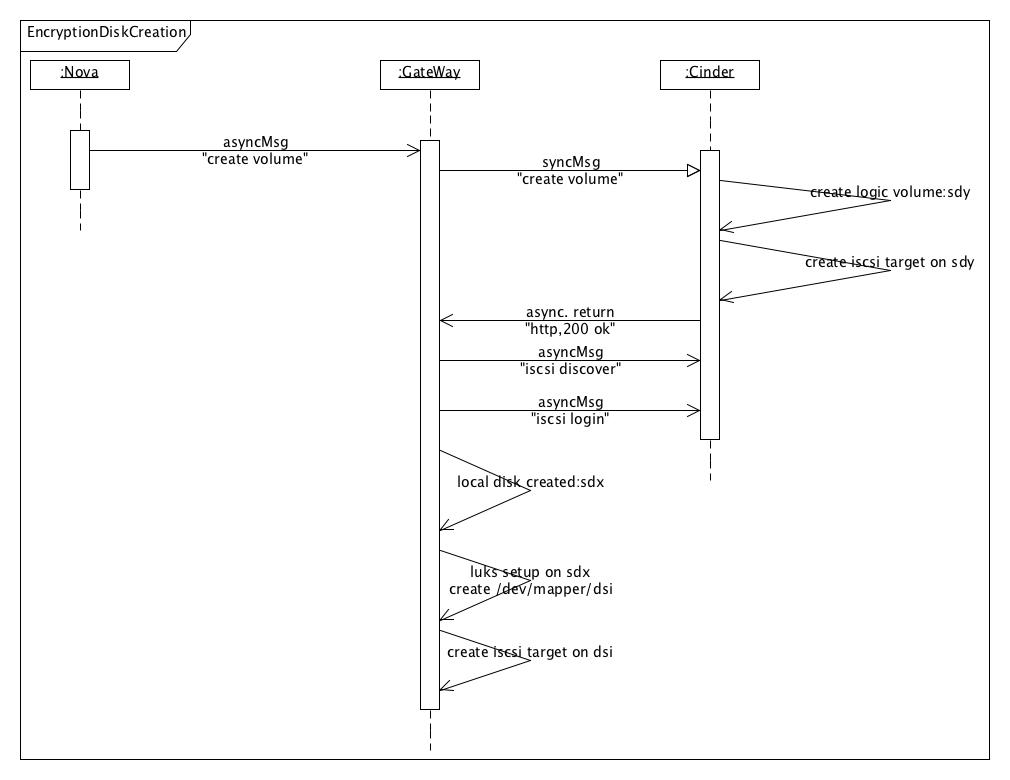
\includegraphics[width=\textwidth,height=170pt,keepaspectratio] {sequence(nova-gw-cinder)}
				\caption{Sequence: create volume nova to gateway to cinder}
				\label{seqngc}
				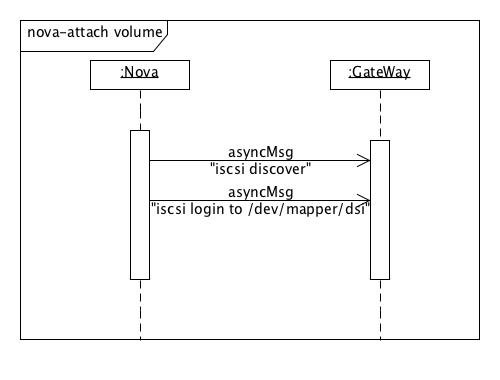
\includegraphics[width=\textwidth,height=140pt,keepaspectratio] {sequence(nova-attach-gw)}
				\caption{Sequence: attach volume, nova to gateway}
				\label{seqng}
			\end{figure}		
			\newpage
			\subsection{Comparison among other possible solution}
			Volume encryption project \cite{volumeencryptionwiki} modify nova side, the encryption volume creation happened in nova side during volume attach, the advantage is easy to implement and possibly better performance, the disadvantage is nova as the resource intended node getting additional stress after this upgrading. In stead of it, our solution of a proxy server can eliminate this problem as we can shift the stress to another/ multiple servers, besides, we can integrate hardware encryption engine into, further reduce the server stress.\\
		\section{Conclusion and Future Works}
			We have proposed a new cloud security storage framework. We have implement the first version as a prototype. The possible future work could be modify horizon in order to support UI-based encryption volume creation( as so far, all in shell command); and integrate hardware engine\cite{Ren13} into it.
			
	%+Bibliography
	%-Bibliography
	\bibliography{REPORTBIB}
	\end{document}